\documentclass[11pt]{article}
\usepackage[T1]{fontenc}
\usepackage[utf8]{inputenc}
\usepackage[
    left=1in,
    right=1in,
    top=0.6in,
    bottom=1in
]{geometry}

\usepackage{amsmath,amssymb}
\usepackage{graphicx}
\usepackage{booktabs}
\usepackage{float}
\usepackage[hidelinks]{hyperref}
\usepackage{tabularx}
\usepackage{caption}
\captionsetup[figure]{font=small}
\usepackage{tikz}
\usetikzlibrary{arrows.meta, positioning}
\usepackage{pgfplots}
\pgfplotsset{compat=1.18}
\setlength{\emergencystretch}{3em}


% Latency chart colours, light to dark, and the UR setting in grey.
\definecolor{latA}{HTML}{A9CDD8}
\definecolor{latB}{HTML}{6FA5B5}
\definecolor{latC}{HTML}{3A7C96}
\definecolor{latD}{HTML}{1E4A66}
\definecolor{latE}{HTML}{BDBDBD}

% File links point to the GitLab repository, branch teleop-refactor.

\title{Week8 Status Report}
\author{Yiran Liu, To: Dr.Pengcheng Xi}
\date{\today}

\begin{document}
\maketitle

\section{Teleoperation Refactor}

Four major stages were outlined in the refactor plan \href{https://gitlabc.nrc-cnrc.gc.ca/Yiran.Liu/nrc_robot_manipulation/-/blob/teleop-refactor/Documentation/Journal/2026Sep/TeleopRefactor.md}{\texttt{TeleopRefactor.md}}. All of them are completed and tested on hardware by now. The camera recording process now stores the video at full resolution and frame rate (480p@30fps), and time-stamps each frame for accurate playback. 

\begin{table}[H]
\centering\small
\begin{tabularx}{\linewidth}{@{}c>{\raggedright\arraybackslash}X>{\raggedright\arraybackslash}p{0.33\linewidth}@{}}
\toprule
Stage & Delivers & Status \\
\midrule
1 & Haply Inverse3 and the 500\,Hz RTDE control loop
  & Latency improvement confirmed \\
2 & Robotiq gripper in its own process
  & Tested on hardware \\
3 & Force sensor reading process at 2\,kHz
  & Tested on Hardware  \\
4 & Cameras: Separate process, time-stamped frames
  & Tested on Hardware (30fps) \\
5 & Force feedback.
  & Has been worked on by Geoffrey. \\
\bottomrule
\end{tabularx}
\end{table}

\section{Inference \& Training Refactor}
\label{sec:policy}

The plan proposed last week
\href{https://gitlabc.nrc-cnrc.gc.ca/Yiran.Liu/nrc_robot_manipulation/-/blob/teleop-refactor/Documentation/Journal/2026Oct/PolicyRefactor.md}{\texttt{PolicyRefactor.md}}, also available on Teams as an editable document, had been caried out.

\subsection{Dashboard and Dataset Trimming}
I proposed to develop a unified visualization dashboard for data transparency. It is used to inspect both the dataset episodes and policy outputs. The dashboard reads CycleLog, our custom lossless logging format. 

\begin{figure}[H]
\centering
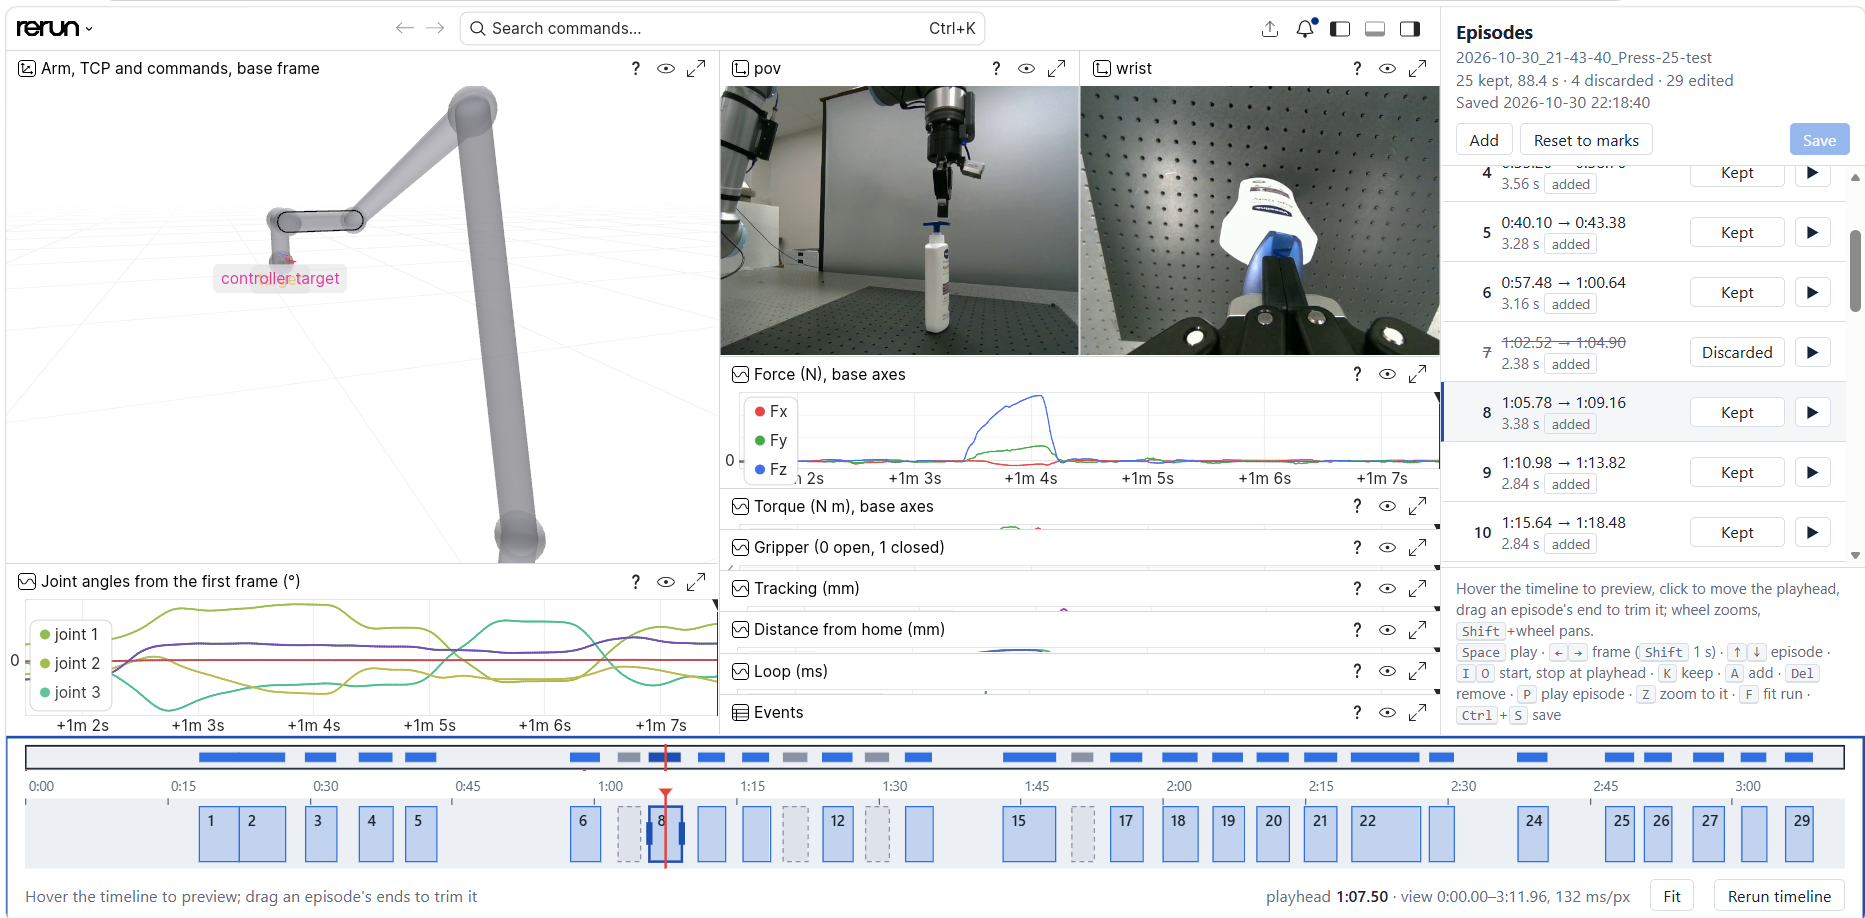
\includegraphics[width=0.75\linewidth]{./Trimming.png}
\end{figure}

This also allows us to redesign how episodes are collected. In the legacy code, we start, save, and drop episodes directly when operating the robot, which makes it possible for mistakes in the dataset. In this dashboard, you can adjust the trimming and drop episodes in the timeline after the collection is done. 

\subsection{LeRobot Model Test on Legacy Dataset}

The usable datasets for the pressing task are in the legacy ZARR format. 
I asked an agent to try to convert them to the LeRobot format. 
It succeeded, though the quality is not fully promised. 
It still allowed me to try training LeRobot's DiffusionPolicy model. 
The training converges with a healthy training curve, producing our first usable LeRobot checkpoint.

\begin{figure}[H]
\centering
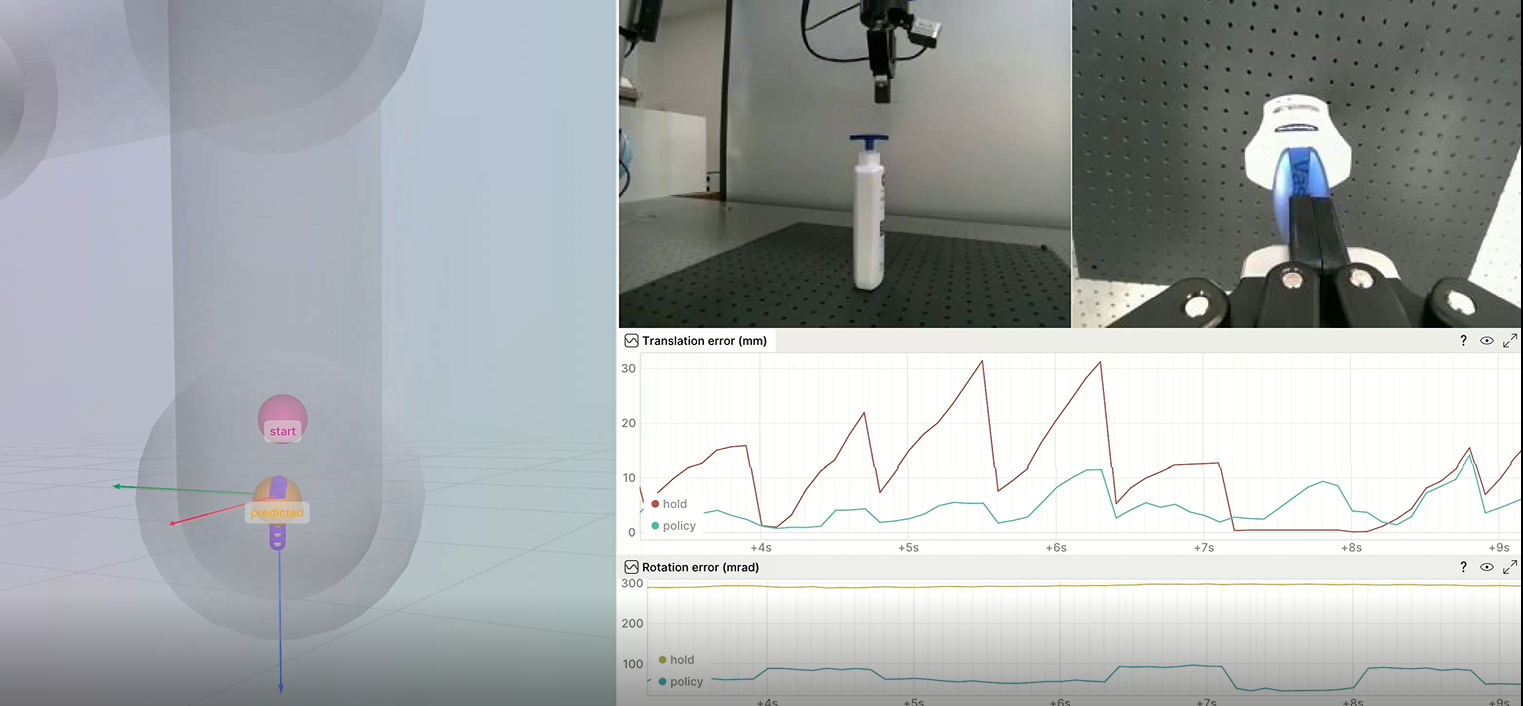
\includegraphics[width=0.80\linewidth]{./DryInference.png}
\end{figure}

I tested the checkpoints in dry-inference runs: I feed the model with frozen frames in a collected episode, and visualize its trajectory output. The action trajectories are reasonable and fit the operator's demonstration. This gives me fair confidence that LeRobot's model and inference runtime will work great on our setup.

\subsection{LeRobot Code Integration}

I installed LeRobot runtime alongside our codebase, now working to adapt it as inference backend for our system:

\begin{enumerate}\label{sec:policy}
  \item (Done) \textbf{Dataset Convention.} Defined the action dimensions and force representation of our dataset within LeRobot's standard. 
  \item (Done) \textbf{Training Script.} One unified training script based on LeRobot's training infrastructure, suiting any model type and with adjustable training settings.
  \item (In-Progress) \textbf{Policy refactor.} Write the contract classes as planned to define boundaries, then write the wrapper code to use LeRobot as inference backend for our codebase.
\end{enumerate}



\section{Plan for Next Week}

\begin{enumerate}\label{sec:plan}
  \item (Team) \textbf{Data Collection. } Collect data using the updated teleop code.
  \item (Team) \textbf{Another Training.} Using the formal dataset convention and newly collected data. 
  \item (Me) \textbf{Robot Execution.} Sending commands according to the trajectory output to roll out the policy.
\end{enumerate}

\end{document}
